\begin{figure}[H]
  \centering
  \begin{subfigure}[t]{.48\linewidth}
    \centering
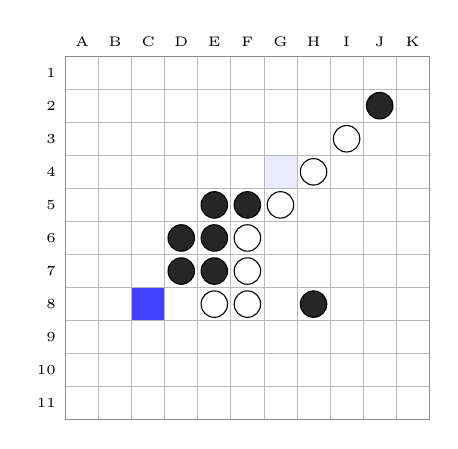
\begin{tikzpicture}[x=0.42cm, y=0.42cm]
\fill[blue!8] (6,-3) rectangle (7,-4);
\fill[blue!75] (2,-7) rectangle (3,-8);
\draw[gray!55, line width=.3pt, step=1] (0,0) grid (11,-11);
\draw[gray!90] (0,0) rectangle (11,-11);
\node[font=\tiny, anchor=south] at (0.5,0) {A};
\node[font=\tiny, anchor=south] at (1.5,0) {B};
\node[font=\tiny, anchor=south] at (2.5,0) {C};
\node[font=\tiny, anchor=south] at (3.5,0) {D};
\node[font=\tiny, anchor=south] at (4.5,0) {E};
\node[font=\tiny, anchor=south] at (5.5,0) {F};
\node[font=\tiny, anchor=south] at (6.5,0) {G};
\node[font=\tiny, anchor=south] at (7.5,0) {H};
\node[font=\tiny, anchor=south] at (8.5,0) {I};
\node[font=\tiny, anchor=south] at (9.5,0) {J};
\node[font=\tiny, anchor=south] at (10.5,0) {K};
\node[font=\tiny, anchor=east] at (0,-0.5) {1};
\node[font=\tiny, anchor=east] at (0,-1.5) {2};
\node[font=\tiny, anchor=east] at (0,-2.5) {3};
\node[font=\tiny, anchor=east] at (0,-3.5) {4};
\node[font=\tiny, anchor=east] at (0,-4.5) {5};
\node[font=\tiny, anchor=east] at (0,-5.5) {6};
\node[font=\tiny, anchor=east] at (0,-6.5) {7};
\node[font=\tiny, anchor=east] at (0,-7.5) {8};
\node[font=\tiny, anchor=east] at (0,-8.5) {9};
\node[font=\tiny, anchor=east] at (0,-9.5) {10};
\node[font=\tiny, anchor=east] at (0,-10.5) {11};
\draw[fill=black!85, line width=.4pt] (9.5,-1.5) circle (.40);
\draw[fill=white, line width=.4pt] (8.5,-2.5) circle (.40);
\draw[fill=white, line width=.4pt] (7.5,-3.5) circle (.40);
\draw[fill=black!85, line width=.4pt] (4.5,-4.5) circle (.40);
\draw[fill=black!85, line width=.4pt] (5.5,-4.5) circle (.40);
\draw[fill=white, line width=.4pt] (6.5,-4.5) circle (.40);
\draw[fill=black!85, line width=.4pt] (3.5,-5.5) circle (.40);
\draw[fill=black!85, line width=.4pt] (4.5,-5.5) circle (.40);
\draw[fill=white, line width=.4pt] (5.5,-5.5) circle (.40);
\draw[fill=black!85, line width=.4pt] (3.5,-6.5) circle (.40);
\draw[fill=black!85, line width=.4pt] (4.5,-6.5) circle (.40);
\draw[fill=white, line width=.4pt] (5.5,-6.5) circle (.40);
\draw[fill=white, line width=.4pt] (4.5,-7.5) circle (.40);
\draw[fill=white, line width=.4pt] (5.5,-7.5) circle (.40);
\draw[fill=black!85, line width=.4pt] (7.5,-7.5) circle (.40);
\end{tikzpicture}
    \caption{SL v3: $v=0{,}18$; đáp án 99,9\%; cao nhất C8 (90,4\%)}
  \end{subfigure}\hfill
  \begin{subfigure}[t]{.48\linewidth}
    \centering
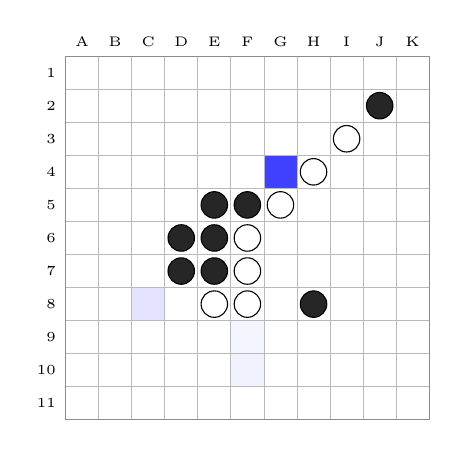
\begin{tikzpicture}[x=0.42cm, y=0.42cm]
\fill[blue!75] (6,-3) rectangle (7,-4);
\fill[blue!11] (2,-7) rectangle (3,-8);
\fill[blue!4] (5,-8) rectangle (6,-9);
\fill[blue!5] (5,-9) rectangle (6,-10);
\draw[gray!55, line width=.3pt, step=1] (0,0) grid (11,-11);
\draw[gray!90] (0,0) rectangle (11,-11);
\node[font=\tiny, anchor=south] at (0.5,0) {A};
\node[font=\tiny, anchor=south] at (1.5,0) {B};
\node[font=\tiny, anchor=south] at (2.5,0) {C};
\node[font=\tiny, anchor=south] at (3.5,0) {D};
\node[font=\tiny, anchor=south] at (4.5,0) {E};
\node[font=\tiny, anchor=south] at (5.5,0) {F};
\node[font=\tiny, anchor=south] at (6.5,0) {G};
\node[font=\tiny, anchor=south] at (7.5,0) {H};
\node[font=\tiny, anchor=south] at (8.5,0) {I};
\node[font=\tiny, anchor=south] at (9.5,0) {J};
\node[font=\tiny, anchor=south] at (10.5,0) {K};
\node[font=\tiny, anchor=east] at (0,-0.5) {1};
\node[font=\tiny, anchor=east] at (0,-1.5) {2};
\node[font=\tiny, anchor=east] at (0,-2.5) {3};
\node[font=\tiny, anchor=east] at (0,-3.5) {4};
\node[font=\tiny, anchor=east] at (0,-4.5) {5};
\node[font=\tiny, anchor=east] at (0,-5.5) {6};
\node[font=\tiny, anchor=east] at (0,-6.5) {7};
\node[font=\tiny, anchor=east] at (0,-7.5) {8};
\node[font=\tiny, anchor=east] at (0,-8.5) {9};
\node[font=\tiny, anchor=east] at (0,-9.5) {10};
\node[font=\tiny, anchor=east] at (0,-10.5) {11};
\draw[fill=black!85, line width=.4pt] (9.5,-1.5) circle (.40);
\draw[fill=white, line width=.4pt] (8.5,-2.5) circle (.40);
\draw[fill=white, line width=.4pt] (7.5,-3.5) circle (.40);
\draw[fill=black!85, line width=.4pt] (4.5,-4.5) circle (.40);
\draw[fill=black!85, line width=.4pt] (5.5,-4.5) circle (.40);
\draw[fill=white, line width=.4pt] (6.5,-4.5) circle (.40);
\draw[fill=black!85, line width=.4pt] (3.5,-5.5) circle (.40);
\draw[fill=black!85, line width=.4pt] (4.5,-5.5) circle (.40);
\draw[fill=white, line width=.4pt] (5.5,-5.5) circle (.40);
\draw[fill=black!85, line width=.4pt] (3.5,-6.5) circle (.40);
\draw[fill=black!85, line width=.4pt] (4.5,-6.5) circle (.40);
\draw[fill=white, line width=.4pt] (5.5,-6.5) circle (.40);
\draw[fill=white, line width=.4pt] (4.5,-7.5) circle (.40);
\draw[fill=white, line width=.4pt] (5.5,-7.5) circle (.40);
\draw[fill=black!85, line width=.4pt] (7.5,-7.5) circle (.40);
\end{tikzpicture}
    \caption{SL không aug: $v=-0{,}42$; đáp án 98,5\%; cao nhất G4 (78,0\%)}
  \end{subfigure}\par\medskip
  \begin{subfigure}[t]{.48\linewidth}
    \centering
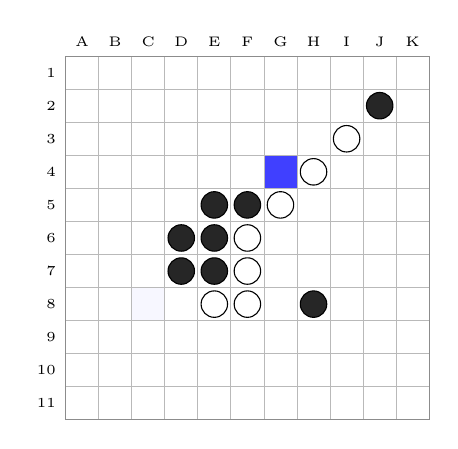
\begin{tikzpicture}[x=0.42cm, y=0.42cm]
\fill[blue!75] (6,-3) rectangle (7,-4);
\fill[blue!3] (2,-7) rectangle (3,-8);
\draw[gray!55, line width=.3pt, step=1] (0,0) grid (11,-11);
\draw[gray!90] (0,0) rectangle (11,-11);
\node[font=\tiny, anchor=south] at (0.5,0) {A};
\node[font=\tiny, anchor=south] at (1.5,0) {B};
\node[font=\tiny, anchor=south] at (2.5,0) {C};
\node[font=\tiny, anchor=south] at (3.5,0) {D};
\node[font=\tiny, anchor=south] at (4.5,0) {E};
\node[font=\tiny, anchor=south] at (5.5,0) {F};
\node[font=\tiny, anchor=south] at (6.5,0) {G};
\node[font=\tiny, anchor=south] at (7.5,0) {H};
\node[font=\tiny, anchor=south] at (8.5,0) {I};
\node[font=\tiny, anchor=south] at (9.5,0) {J};
\node[font=\tiny, anchor=south] at (10.5,0) {K};
\node[font=\tiny, anchor=east] at (0,-0.5) {1};
\node[font=\tiny, anchor=east] at (0,-1.5) {2};
\node[font=\tiny, anchor=east] at (0,-2.5) {3};
\node[font=\tiny, anchor=east] at (0,-3.5) {4};
\node[font=\tiny, anchor=east] at (0,-4.5) {5};
\node[font=\tiny, anchor=east] at (0,-5.5) {6};
\node[font=\tiny, anchor=east] at (0,-6.5) {7};
\node[font=\tiny, anchor=east] at (0,-7.5) {8};
\node[font=\tiny, anchor=east] at (0,-8.5) {9};
\node[font=\tiny, anchor=east] at (0,-9.5) {10};
\node[font=\tiny, anchor=east] at (0,-10.5) {11};
\draw[fill=black!85, line width=.4pt] (9.5,-1.5) circle (.40);
\draw[fill=white, line width=.4pt] (8.5,-2.5) circle (.40);
\draw[fill=white, line width=.4pt] (7.5,-3.5) circle (.40);
\draw[fill=black!85, line width=.4pt] (4.5,-4.5) circle (.40);
\draw[fill=black!85, line width=.4pt] (5.5,-4.5) circle (.40);
\draw[fill=white, line width=.4pt] (6.5,-4.5) circle (.40);
\draw[fill=black!85, line width=.4pt] (3.5,-5.5) circle (.40);
\draw[fill=black!85, line width=.4pt] (4.5,-5.5) circle (.40);
\draw[fill=white, line width=.4pt] (5.5,-5.5) circle (.40);
\draw[fill=black!85, line width=.4pt] (3.5,-6.5) circle (.40);
\draw[fill=black!85, line width=.4pt] (4.5,-6.5) circle (.40);
\draw[fill=white, line width=.4pt] (5.5,-6.5) circle (.40);
\draw[fill=white, line width=.4pt] (4.5,-7.5) circle (.40);
\draw[fill=white, line width=.4pt] (5.5,-7.5) circle (.40);
\draw[fill=black!85, line width=.4pt] (7.5,-7.5) circle (.40);
\end{tikzpicture}
    \caption{L6 (RL): $v=0{,}19$; đáp án 100,0\%; cao nhất G4 (95,6\%)}
  \end{subfigure}\hfill
  \begin{subfigure}[t]{.48\linewidth}
    \centering
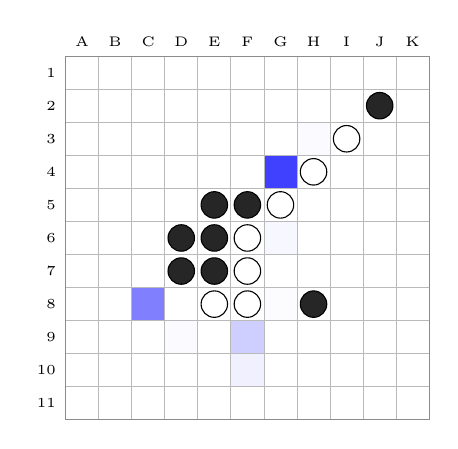
\begin{tikzpicture}[x=0.42cm, y=0.42cm]
\fill[blue!2] (7,-2) rectangle (8,-3);
\fill[blue!75] (6,-3) rectangle (7,-4);
\fill[blue!3] (6,-5) rectangle (7,-6);
\fill[blue!50] (2,-7) rectangle (3,-8);
\fill[blue!1] (6,-7) rectangle (7,-8);
\fill[blue!2] (3,-8) rectangle (4,-9);
\fill[blue!19] (5,-8) rectangle (6,-9);
\fill[blue!6] (5,-9) rectangle (6,-10);
\draw[gray!55, line width=.3pt, step=1] (0,0) grid (11,-11);
\draw[gray!90] (0,0) rectangle (11,-11);
\node[font=\tiny, anchor=south] at (0.5,0) {A};
\node[font=\tiny, anchor=south] at (1.5,0) {B};
\node[font=\tiny, anchor=south] at (2.5,0) {C};
\node[font=\tiny, anchor=south] at (3.5,0) {D};
\node[font=\tiny, anchor=south] at (4.5,0) {E};
\node[font=\tiny, anchor=south] at (5.5,0) {F};
\node[font=\tiny, anchor=south] at (6.5,0) {G};
\node[font=\tiny, anchor=south] at (7.5,0) {H};
\node[font=\tiny, anchor=south] at (8.5,0) {I};
\node[font=\tiny, anchor=south] at (9.5,0) {J};
\node[font=\tiny, anchor=south] at (10.5,0) {K};
\node[font=\tiny, anchor=east] at (0,-0.5) {1};
\node[font=\tiny, anchor=east] at (0,-1.5) {2};
\node[font=\tiny, anchor=east] at (0,-2.5) {3};
\node[font=\tiny, anchor=east] at (0,-3.5) {4};
\node[font=\tiny, anchor=east] at (0,-4.5) {5};
\node[font=\tiny, anchor=east] at (0,-5.5) {6};
\node[font=\tiny, anchor=east] at (0,-6.5) {7};
\node[font=\tiny, anchor=east] at (0,-7.5) {8};
\node[font=\tiny, anchor=east] at (0,-8.5) {9};
\node[font=\tiny, anchor=east] at (0,-9.5) {10};
\node[font=\tiny, anchor=east] at (0,-10.5) {11};
\draw[fill=black!85, line width=.4pt] (9.5,-1.5) circle (.40);
\draw[fill=white, line width=.4pt] (8.5,-2.5) circle (.40);
\draw[fill=white, line width=.4pt] (7.5,-3.5) circle (.40);
\draw[fill=black!85, line width=.4pt] (4.5,-4.5) circle (.40);
\draw[fill=black!85, line width=.4pt] (5.5,-4.5) circle (.40);
\draw[fill=white, line width=.4pt] (6.5,-4.5) circle (.40);
\draw[fill=black!85, line width=.4pt] (3.5,-5.5) circle (.40);
\draw[fill=black!85, line width=.4pt] (4.5,-5.5) circle (.40);
\draw[fill=white, line width=.4pt] (5.5,-5.5) circle (.40);
\draw[fill=black!85, line width=.4pt] (3.5,-6.5) circle (.40);
\draw[fill=black!85, line width=.4pt] (4.5,-6.5) circle (.40);
\draw[fill=white, line width=.4pt] (5.5,-6.5) circle (.40);
\draw[fill=white, line width=.4pt] (4.5,-7.5) circle (.40);
\draw[fill=white, line width=.4pt] (5.5,-7.5) circle (.40);
\draw[fill=black!85, line width=.4pt] (7.5,-7.5) circle (.40);
\end{tikzpicture}
    \caption{L8 (AZ): $v=-0{,}78$; đáp án 64,4\%; cao nhất G4 (32,3\%)}
  \end{subfigure}\par\medskip
  \caption{Policy của bốn mạng tại thế C5-001 (O đi). Ô càng đậm xác suất càng cao (chuẩn hoá theo ô lớn nhất của từng mạng). Đáp án: G4, C8, F9, F10.}
  \label{fig:cs-policy-c5}
\end{figure}
